\subsection{Fase PROB}
	\textbf{Periodo}: dal \insdate{16}{03}{2015} al \insdate{08}{04}{2015} \\Questa fase comincia con la fine della \insphase{Fase PA} e termina con l'incontro con il proponente al fine di mostrare il prototipo con i requisiti obbligatori sviluppati.\\Le attività di questa fase saranno le seguenti:
	\begin{itemize}
		\item\textbf{Definizione di Prodotto}: Viene steso il documento \insfile{Definizione di Prodotto 1.0}. Esso definisce la struttura interna del sistema e le relazioni dei componenti del prodotto relativi ai requisiti obbligatori.
		\item\textbf{Manuale Utente e Manuale Amministratore}: Comincia la stesura dei manuali che forniranno indicazioni agli utilizzatori del sistema.
		\item\textbf{Incremento e Verifica Documenti}: Vengono eseguite modifiche ai documenti già scritti, se necessario.
		\item\textbf{Glossario}: Vengono aggiunti al file \insfile{Glossario.xml} i vocaboli dei quali si ritiene necessaria una definizione formale. Alla fine di questa fase vieni quindi generato il documento \insdoc{Glossario 4.0}.
	\end{itemize}
	\subsubsection{Diagramma di Gantt delle attività}
		%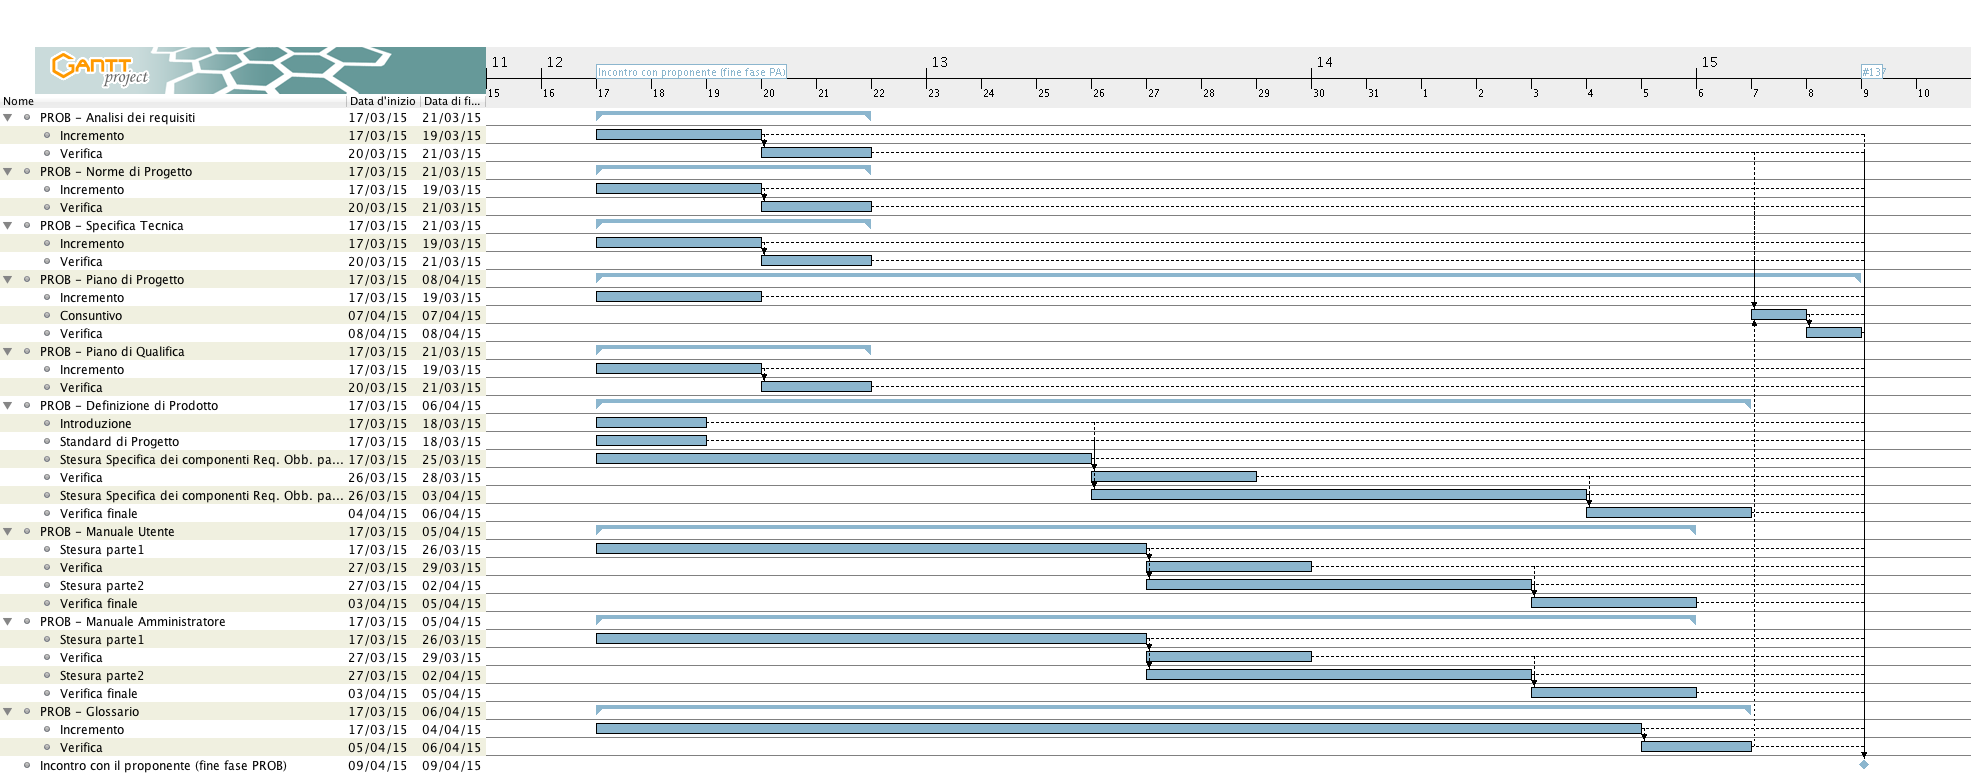
\includegraphics{PianoDiProgetto/Pics/FasePROB.png}